%
% lagrangezyl.tex
%
% (c) 2021 Prof Dr Andreas Müller, OST Ostschweizer Fachhochschule
%
\documentclass[tikz]{standalone}
\usepackage{times}
\usepackage{amsmath}
\usepackage{txfonts}
\usepackage[utf8]{inputenc}
\usepackage{graphics}
\usetikzlibrary{arrows,intersections,math,calc}
\usepackage{ifthen}
\begin{document}

\newboolean{showgrid}
\setboolean{showgrid}{false}
\def\breite{7}
\def\hoehe{4}

\begin{tikzpicture}[>=latex,thick]
\clip (-6.3,-4) rectangle (6.3,4);

% Povray Bild
\node at (0,0) {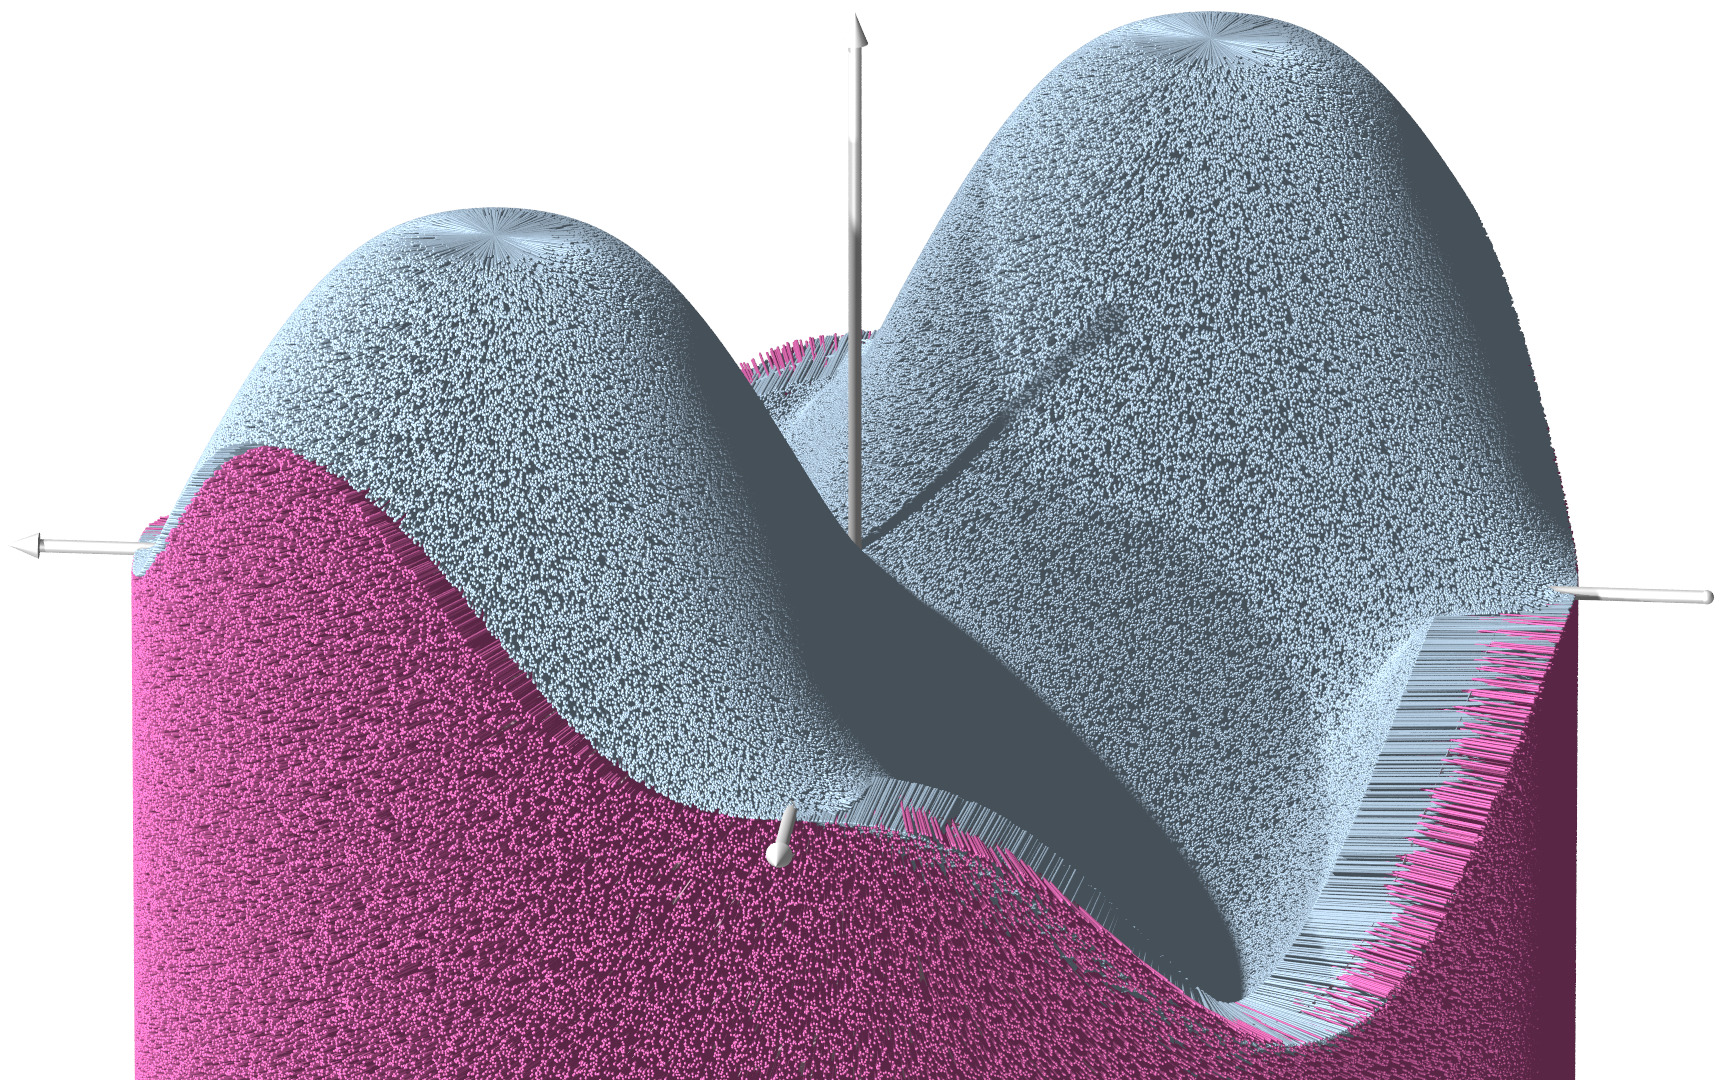
\includegraphics[width=12.6cm]{lagrangezyl.jpg}};

% Gitter
\ifthenelse{\boolean{showgrid}}{
\draw[step=0.1,line width=0.1pt] (-\breite,-\hoehe) grid (\breite, \hoehe);
\draw[step=0.5,line width=0.4pt] (-\breite,-\hoehe) grid (\breite, \hoehe);
\draw                            (-\breite,-\hoehe) grid (\breite, \hoehe);
\fill (0,0) circle[radius=0.05];
}{}


\node at (-6.1,0.2) {$x$};
\coordinate (Y) at (-0.6,-2.65);
\fill[color=white,opacity=0.5] ($(Y)+(-0.15,-0.2)$) rectangle +(0.3,0.4);
\node at (Y) {$y$};
\node at (-0.2,3.8) {$z$};

\end{tikzpicture}

\end{document}
